

\section{Programstruktur}
Baseret på de førnævnte krav blev designfasen påbegyndt. Målet var at forsimple opgaven for brugeren så meget som overhoved muligt, da det ikke vil kunne forvæntes at denne person kender noget til det bagvedlæggende system. 
Tilsvarende ønskes der en simpel og generel anvendelse af programmets services fra de høje lag nær chat-klienten, hvor de mere administrative og praktiske funktionaliteter skal håndteres længere nede i systemet.

\begin{figure}[h!]
\centering
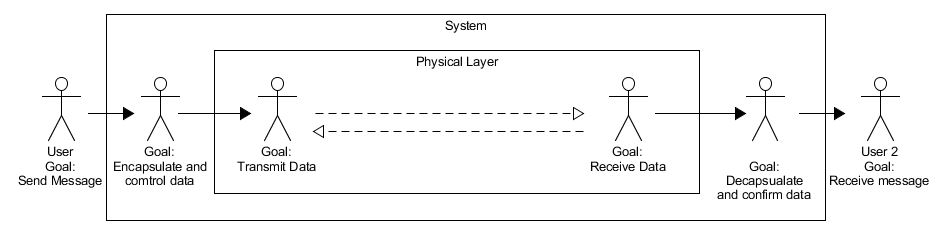
\includegraphics[scale=0.5]{Billeder/ProgramOpbygning1.JPG}
\caption{System opbygning - første udkast}
\label{fig:Blokdiagram}
\end{figure}

Figur \ref{fig:Blokdiagram} viser første udkast til programmets struktur i grove træk. Afsenderen modtager data fra brugeren, og indkapsler dette i en format modtageren er i stand til at forstå. Herfra tager det næste lag sig ad den reelle transmission og afkodning af informationen. Dette lag er upålideligt, så modtageren skal tilsvarende her validere indholdet og rækkefølgen af informationen får at kunne sikre at informationen når korrekt frem til brugeren. 

I og med at den ønskede applikation er et chat-program, er det af høj prioritet, at den logiske forbindelse mellem de to brugere er pålidelig. Dette indebære at det som afsenderen skriver skal være præcis det samme som modtageren læser. Systemet vil derfor tage udgangspunkt i TCP/IP, da denne protokol vigtigst af alt tilbyder en pålidelig overførsel af data. 




\subsection{Klassediagram}
Hvordan skal en domænemodel opbygges for at sikre denne karakteristik. 

Jeg 

Baseret på krav og domænemodel tilføjes nu funktionalitet

Jævnføre projektoplæget skal der anvendes en lagsopdelt arkitektur. 

det viste klassediagram er et udkast til programmet, og kan derfor ændre sig efter behov gennem projektet. nedenstående.


\subsection{Ansvarsfordeling til klasser}
Hvordan forvæntes de forskellige “sorte kasser” at arbejde sammen (grænse flader)

-Udpenslende forklaring af ansvarsfordeling og programstruktur.  

Derfor vil opgraderinger i konverteringen på applikationslaget være nok til at lade systemet understøtte flere datatyper (billeder, lyd og filer)